\documentclass{standalone}
\usepackage{tikz}
\usepackage{graphicx} % For rotatebox
\usetikzlibrary{circuits.ee.IEC, decorations.markings}

\begin{document}
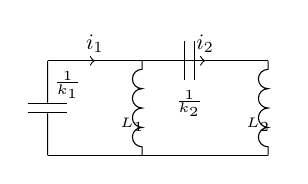
\begin{tikzpicture}[circuit ee IEC, scale=0.8, transform shape]

% Define components
\def\kone{2} % Capacitance 1/k1
\def\ktwo{3} % Capacitance 1/k2
\def\lone{1.5} % Inductance L1
\def\ltwo{1.8} % Inductance L2

% Draw parallel combination
\draw[fill=gray!30] (0,0) to [inductor={info={\rotatebox{270}{\tiny$L_1$}}, align=center}] ++(0,1.5) coordinate (L1);
\draw[fill=gray!30] (-1.5,0) to [capacitor={info'={\rotatebox{270}{\tiny$\frac{1}{k_1}$}}, swap, align=center}] ++(0,1.5) coordinate (C1);

% Add series combination
\draw[fill=gray!30] (0,1.5) coordinate (C2start) to [capacitor={info'={\rotatebox{0}{\tiny$\frac{1}{k_2}$}}, swap, align=center}] ++(1.5,0) coordinate (C2end);
\draw[fill=gray!30] (2,0) to [inductor={info={\rotatebox{270}{\tiny$L_2$}}, align=center}] ++(0,1.5) coordinate (L2);

% Draw lines connecting components

\draw (-1.5,0) -- (2,0);

% Add pointer and label for i1
\draw[postaction={decorate,decoration={markings,mark=at position 0.5 with {\arrow{>}}}}] (-1.5,1.5) -- node[above] {\(i_1\)} (0,1.5);

% Add pointer and label for i2
\draw[postaction={decorate,decoration={markings,mark=at position 0.5 with {\arrow{>}}}}] (0,1.5) -- node[above] {\(i_2\)} (2,1.5);
\end{tikzpicture}
\end{document}

